% Options for packages loaded elsewhere
\PassOptionsToPackage{unicode}{hyperref}
\PassOptionsToPackage{hyphens}{url}
\documentclass[
  11pt,
]{article}
\usepackage{xcolor}
\usepackage[margin=1in]{geometry}
\usepackage{amsmath,amssymb}
\setcounter{secnumdepth}{5}
\usepackage{iftex}
\ifPDFTeX
  \usepackage[T1]{fontenc}
  \usepackage[utf8]{inputenc}
  \usepackage{textcomp} % provide euro and other symbols
\else % if luatex or xetex
  \usepackage{unicode-math} % this also loads fontspec
  \defaultfontfeatures{Scale=MatchLowercase}
  \defaultfontfeatures[\rmfamily]{Ligatures=TeX,Scale=1}
\fi
\usepackage{lmodern}
\ifPDFTeX\else
  % xetex/luatex font selection
\fi
% Use upquote if available, for straight quotes in verbatim environments
\IfFileExists{upquote.sty}{\usepackage{upquote}}{}
\IfFileExists{microtype.sty}{% use microtype if available
  \usepackage[]{microtype}
  \UseMicrotypeSet[protrusion]{basicmath} % disable protrusion for tt fonts
}{}
\makeatletter
\@ifundefined{KOMAClassName}{% if non-KOMA class
  \IfFileExists{parskip.sty}{%
    \usepackage{parskip}
  }{% else
    \setlength{\parindent}{0pt}
    \setlength{\parskip}{6pt plus 2pt minus 1pt}}
}{% if KOMA class
  \KOMAoptions{parskip=half}}
\makeatother
\usepackage{graphicx}
\makeatletter
\newsavebox\pandoc@box
\newcommand*\pandocbounded[1]{% scales image to fit in text height/width
  \sbox\pandoc@box{#1}%
  \Gscale@div\@tempa{\textheight}{\dimexpr\ht\pandoc@box+\dp\pandoc@box\relax}%
  \Gscale@div\@tempb{\linewidth}{\wd\pandoc@box}%
  \ifdim\@tempb\p@<\@tempa\p@\let\@tempa\@tempb\fi% select the smaller of both
  \ifdim\@tempa\p@<\p@\scalebox{\@tempa}{\usebox\pandoc@box}%
  \else\usebox{\pandoc@box}%
  \fi%
}
% Set default figure placement to htbp
\def\fps@figure{htbp}
\makeatother
% definitions for citeproc citations
\NewDocumentCommand\citeproctext{}{}
\NewDocumentCommand\citeproc{mm}{%
  \begingroup\def\citeproctext{#2}\cite{#1}\endgroup}
\makeatletter
 % allow citations to break across lines
 \let\@cite@ofmt\@firstofone
 % avoid brackets around text for \cite:
 \def\@biblabel#1{}
 \def\@cite#1#2{{#1\if@tempswa , #2\fi}}
\makeatother
\newlength{\cslhangindent}
\setlength{\cslhangindent}{1.5em}
\newlength{\csllabelwidth}
\setlength{\csllabelwidth}{3em}
\newenvironment{CSLReferences}[2] % #1 hanging-indent, #2 entry-spacing
 {\begin{list}{}{%
  \setlength{\itemindent}{0pt}
  \setlength{\leftmargin}{0pt}
  \setlength{\parsep}{0pt}
  % turn on hanging indent if param 1 is 1
  \ifodd #1
   \setlength{\leftmargin}{\cslhangindent}
   \setlength{\itemindent}{-1\cslhangindent}
  \fi
  % set entry spacing
  \setlength{\itemsep}{#2\baselineskip}}}
 {\end{list}}
\usepackage{calc}
\newcommand{\CSLBlock}[1]{\hfill\break\parbox[t]{\linewidth}{\strut\ignorespaces#1\strut}}
\newcommand{\CSLLeftMargin}[1]{\parbox[t]{\csllabelwidth}{\strut#1\strut}}
\newcommand{\CSLRightInline}[1]{\parbox[t]{\linewidth - \csllabelwidth}{\strut#1\strut}}
\newcommand{\CSLIndent}[1]{\hspace{\cslhangindent}#1}
\setlength{\emergencystretch}{3em} % prevent overfull lines
\providecommand{\tightlist}{%
  \setlength{\itemsep}{0pt}\setlength{\parskip}{0pt}}
\usepackage{setspace}
\usepackage{graphicx}
\usepackage{caption}
\doublespacing
\setlength{\parindent}{0pt}
\setlength{\parskip}{1em}
\usepackage{booktabs}
\usepackage{multirow}
\usepackage{bookmark}
\IfFileExists{xurl.sty}{\usepackage{xurl}}{} % add URL line breaks if available
\urlstyle{same}
\hypersetup{
  pdftitle={Effectiveness of Extreme Risk Protection Orders on Firearm Suicide},
  hidelinks,
  pdfcreator={LaTeX via pandoc}}

\title{Effectiveness of Extreme Risk Protection Orders on Firearm
Suicide}
\author{true}
\date{}

\begin{document}
\maketitle

\section{Introduction}\label{introduction}

Firearm suicide is a major public health crisis in the United States,
accounting for more than half of all suicide deaths each year. Men
constitute the vast majority of firearm suicide decedents, and the
lethality of firearms makes attempts with guns far more likely to result
in death than other methods.

Extreme Risk Protection Orders (ERPOs) have emerged as a promising legal
mechanism to temporarily restrict firearm access for individuals deemed
at imminent risk of harm to themselves or others. These civil orders,
enacted in more than 20 states, are designed to interrupt escalating
risk---particularly for individuals experiencing suicidal crises. While
case reports and early evaluations have suggested that ERPOs may be
effective in averting imminent suicide attempts, population-level
evidence on their longer-term effects remains limited and contested.

In this study, we use a Bayesian state-year panel model to evaluate the
effect of ERPO laws on firearm suicide rates. Our analysis spans over
two decades and includes all 50 U.S. states and the District of
Columbia. We hypothesize that the implementation of ERPO laws is
associated with a measurable reduction in firearm suicide, particularly
among men.

\begin{figure}[htbp]
  \centering
  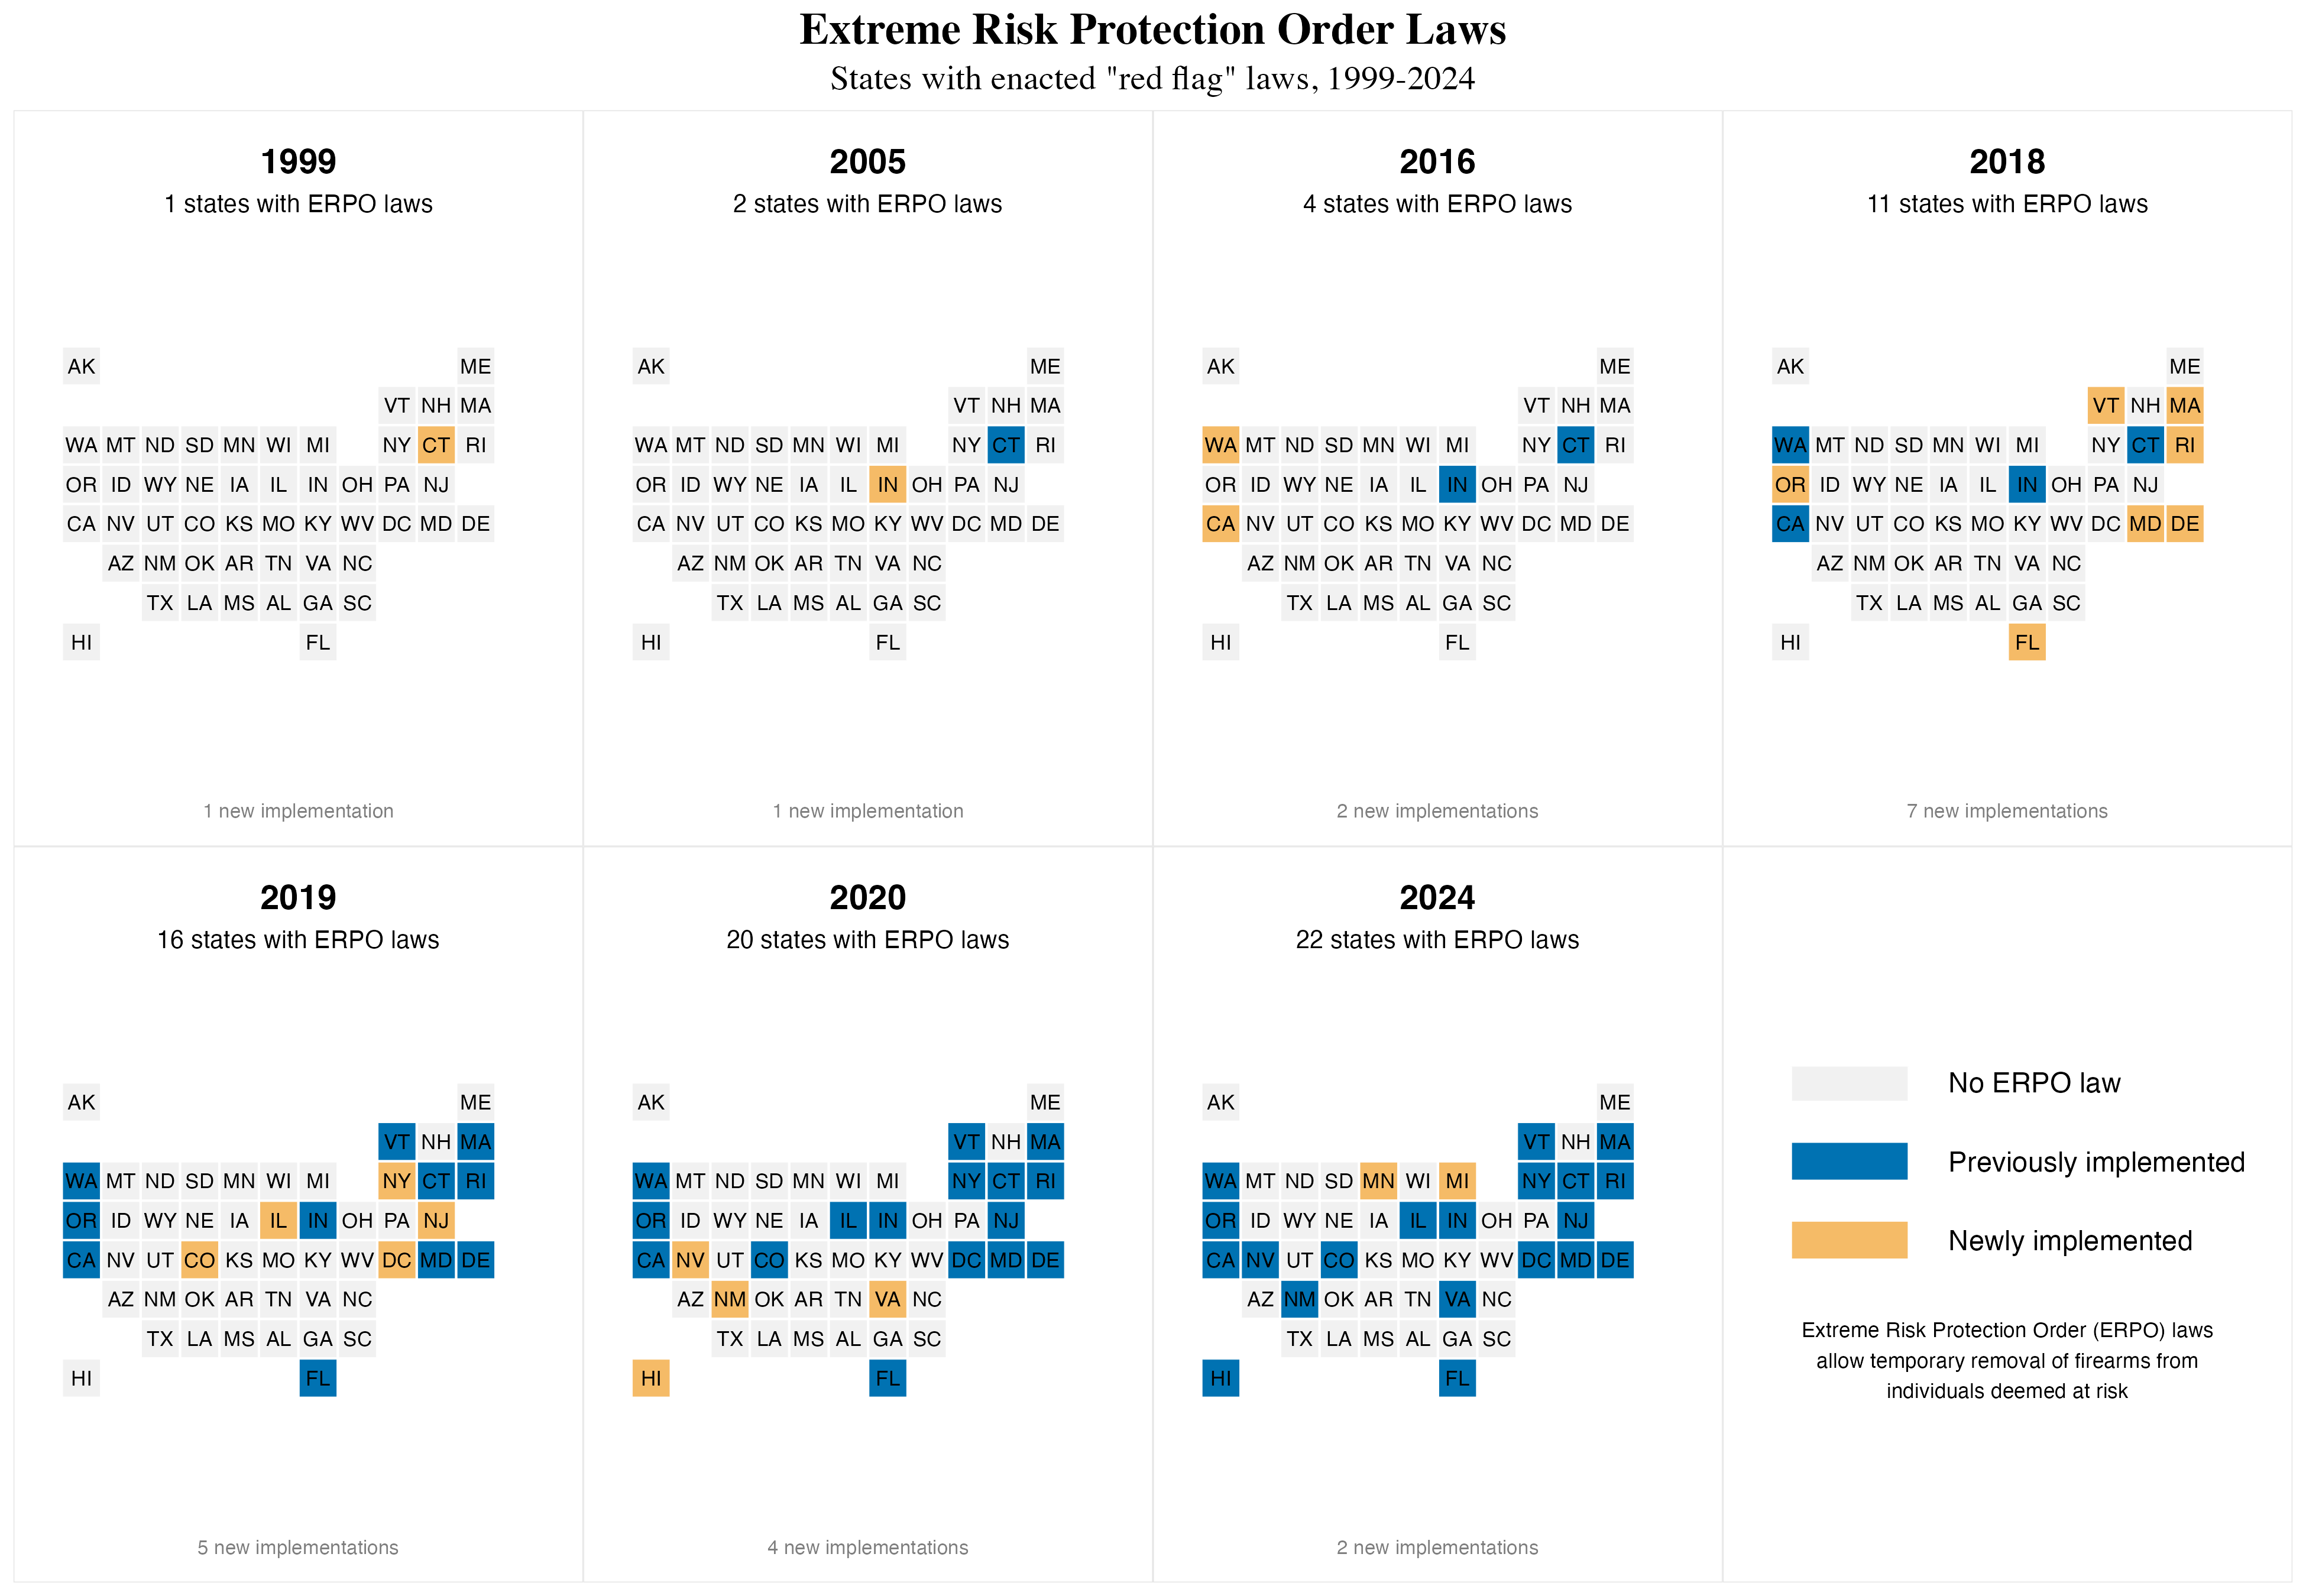
\includegraphics[width=\textwidth]{../erpo_laws_spread.png}
  \caption{
    \textbf{State Implementation of Extreme Risk Protection Order (ERPO) Laws, 1999–2024.}  \\
    \footnotesize\textit{This figure shows the annual spread of ERPO laws across U.S. states from 1999 to 2024. States are color-coded by implementation status: orange indicates states that newly implemented an ERPO law in that year, blue indicates states with previously implemented ERPO laws, and gray indicates states without such laws. ERPO laws allow for the temporary removal of firearms from individuals deemed to be at risk of harming themselves or others. By 2024, 22 states had enacted ERPO legislation.
  }}
  \label{fig:erpo_map}
\end{figure}

\section{Methods}\label{methods}

The study was determined to be exempt from review and from a requirement
for informed consent, because it used no identifiable human participant
data, by the RAND institutional review board. The study follows good
research practices for comparative effectiveness research,15 eg, the
data sources, modeling methods, primary comparisons, and sensitivity
tests were preregistered, and the data and statistical code are
available. The eAppendix in Supplement 1 provides a detailed discussion
of how the current study extends and improves prior published research
by the authors.

\subsection{Data}\label{data}

Mortality data from 1999 to 2023 come from the National Vital Statistics
System, which provides information on coroners' cause of death
determinations for a near-census of deaths in the United States (1),
(2). Information on the effective dates of firearm laws come from the
RAND State Firearm Law Database.18 The analyses also include state-level
demographic, economic, crime, and gun ownership characteristics; sources
for these are described in the eAppendix in Supplement 1.

\subsection{Appendix}\label{appendix}

\begin{table}[ht]
\centering
\caption{Implementation Timeline of Extreme Risk Protection Order Laws by State (as of April 2024)}
\label{tab:erpo_timeline}
\begin{tabular}{lccc}
\toprule
\textbf{State} & \textbf{Effective Date} & \textbf{Year} & \textbf{Years in Effect (as of 2023)} \\
\midrule
Connecticut & October 1, 1999 & 1999 & 24 \\
Indiana & July 1, 2005 & 2005 & 18 \\
California & January 1, 2016 & 2016 & 7 \\
Washington & December 8, 2016 & 2016 & 7 \\
Oregon & January 1, 2018 & 2018 & 5 \\
Vermont & April 11, 2018 & 2018 & 5 \\
Florida & March 9, 2018 & 2018 & 5 \\
Rhode Island & June 1, 2018 & 2018 & 5 \\
Maryland & October 1, 2018 & 2018 & 5 \\
Massachusetts & August 17, 2018 & 2018 & 5 \\
Delaware & December 27, 2018 & 2018 & 5 \\
Illinois & January 1, 2019 & 2019 & 4 \\
Colorado & April 12, 2019 & 2019 & 4 \\
District of Columbia & January 30, 2019 & 2019 & 4 \\
New York & August 24, 2019 & 2019 & 4 \\
New Jersey & September 1, 2019 & 2019 & 4 \\
Hawaii & January 1, 2020 & 2020 & 3 \\
Nevada & January 1, 2020 & 2020 & 3 \\
New Mexico & May 20, 2020 & 2020 & 3 \\
Virginia & July 1, 2020 & 2020 & 3 \\
U.S. Virgin Islands & February 1, 2023 & 2023 & <1 \\
Michigan & February 13, 2024 & 2024 & 0 \\
Minnesota & January 1, 2024 & 2024 & 0 \\
\bottomrule
\multicolumn{4}{p{.97\linewidth}}{\small \textit{Sources:} RAND State Firearm Law Database (2024); Johns Hopkins Center for Gun Violence Solutions (2023); Giffords Law Center (2023).}
\end{tabular}
\end{table}

\clearpage

\begin{table}[ht]
\centering
\caption{Key Policy Features of Extreme Risk Protection Order Laws (as of April 2024)}
\label{tab:erpo_features}
\begin{tabular}{lcccccc}
\toprule
\multirow{2}{*}{\textbf{State}} & \multicolumn{3}{c}{\textbf{Authorized Petitioners}} & \multicolumn{2}{c}{\textbf{Ex Parte Provisions}} & \multirow{2}{*}{\textbf{Final Order}} \\
\cmidrule(lr){2-4} \cmidrule(lr){5-6}
 & \textbf{Law Enf.} & \textbf{Family} & \textbf{Other} & \textbf{Available} & \textbf{Duration (days)} & \textbf{Duration} \\
\midrule
California & \checkmark & \checkmark & \checkmark & \checkmark & 21 & 1-5 years \\
Colorado & \checkmark & \checkmark & \checkmark & \checkmark & 14 & 364 days \\
Connecticut & \checkmark & \checkmark & \checkmark & \checkmark & 14 & Until terminated \\
Delaware & \checkmark & \checkmark & - & \checkmark & 15 & Up to 1 year \\
District of Columbia & \checkmark & \checkmark & \checkmark & \checkmark & 14 & 1 year \\
Florida & \checkmark & - & - & \checkmark & 14 & Up to 1 year \\
Hawaii & \checkmark & \checkmark & \checkmark & \checkmark & 14 & 1 year \\
Illinois & \checkmark & \checkmark & - & \checkmark & 14 & 6 mo. to 1 yr. \\
Indiana & \checkmark & - & - & \checkmark & 14 & Until terminated \\
Maryland & \checkmark & \checkmark & \checkmark & \checkmark & 7 & Up to 1 year \\
Massachusetts & \checkmark & \checkmark & \checkmark & \checkmark & 10 & Up to 1 year \\
Michigan & \checkmark & \checkmark & \checkmark & \checkmark & 14 & 1 year \\
Minnesota & \checkmark & \checkmark & \checkmark & \checkmark & 14 & 6 mo. to 1 yr. \\
Nevada & \checkmark & \checkmark & - & \checkmark & 7 & Up to 1 year \\
New Jersey & \checkmark & \checkmark & - & \checkmark & 10 & Until terminated \\
New Mexico & \checkmark & - & - & \checkmark & 10 & Up to 1 year \\
New York & \checkmark & \checkmark & \checkmark & \checkmark & 6 & Up to 1 year \\
Oregon & \checkmark & \checkmark & - & - & N/A & 1 year \\
Rhode Island & \checkmark & - & - & \checkmark & 14 & 1 year \\
U.S. Virgin Islands & \checkmark & \checkmark & \checkmark & \checkmark & 14 & 1 year \\
Vermont & \checkmark & \checkmark & - & \checkmark & 14 & Up to 6 months \\
Virginia & \checkmark & \checkmark & - & \checkmark & 14 & Up to 180 days \\
Washington & \checkmark & \checkmark & - & \checkmark & 14 & 1 year \\
\bottomrule
\multicolumn{7}{p{.97\linewidth}}{\small \textit{Notes:} "Other" petitioners may include healthcare professionals, educators, co-workers, or state's attorneys, depending on the state. "Law Enf." refers to law enforcement officers. Michigan and Minnesota laws went into effect in 2024.}
\end{tabular}
\end{table}

\clearpage

\begin{table}[ht]
\centering
\caption{Classification of ERPO Laws by Policy Feature Categories (as of April 2024)}
\label{tab:erpo_categories}
\begin{tabular}{lcc}
\toprule
\textbf{Policy Feature} & \textbf{States} & \textbf{Count} \\
\midrule
\textbf{Petitioner Access} & & \\
Law Enforcement Only & Florida, Indiana, New Mexico, Rhode Island & 4 \\
Family Members Included & All other ERPO states & 19 \\
Healthcare Prof. Included & CA, CO, CT, DC, HI, MD, MA, MI, MN, NY, VI & 11 \\
\midrule
\textbf{Ex Parte Provisions} & & \\
Available & All except Oregon & 22 \\
Not Available & Oregon & 1 \\
Short Duration ($\leq$10 days) & MD, MA, NJ, NM, NY, NV & 6 \\
Standard Duration (>10 days) & All others with ex parte & 16 \\
\midrule
\textbf{Final Order Duration} & & \\
6 months or less & Vermont, Virginia & 2 \\
Up to 1 year (standard) & Most states & 18 \\
Until terminated & Connecticut, Indiana, New Jersey & 3 \\
\midrule
\textbf{Implementation Intensity} & & \\
High & Florida, Maryland & 2 \\
Medium & CA, CO, CT, NY, OR, RI, WA & 7 \\
Low & All others & 14 \\
\bottomrule
\multicolumn{3}{p{.95\linewidth}}{\small \textit{Sources:} Data compiled from Johns Hopkins Center for Gun Violence Solutions (2023), RAND State Firearm Law Database (2024), and Giffords Law Center (2023). Implementation intensity categories based on estimated ERPOs per 100,000 population.}
\end{tabular}
\end{table}

\clearpage

\protect\phantomsection\label{refs}
\begin{CSLReferences}{0}{1}
\bibitem[\citeproctext]{ref-cdc2021wonder}
\CSLLeftMargin{1. }%
\CSLRightInline{Centers for Disease Control and Prevention, National
Center for Health Statistics. National vital statistics system,
mortality 1999--2020 on CDC WONDER online database.
\url{https://wonder.cdc.gov/ucd-icd10.html}; 2021. }

\bibitem[\citeproctext]{ref-cdc2024wonder}
\CSLLeftMargin{2. }%
\CSLRightInline{Centers for Disease Control and Prevention, National
Center for Health Statistics. National vital statistics system,
mortality 2018--2023 on CDC WONDER online database.
\url{https://wonder.cdc.gov/ucd-icd10-expanded.html}; 2024. }

\end{CSLReferences}

\end{document}
